\subsection{FUNCTORIAL PROPERTIES}

PROPOSITION 6. Let G, H be Lie groups and \(\phi\) a morphism of G into H. For \(t, t'\) in \(\mathcal{T}^{(\infty)}(G)\) , \(\phi_{*}(t * t') = \phi_{*}(t) * \phi_{*}(t')\) .

Consider the diagram

\[
\begin{array}{c} \mathrm{G} \times \mathrm{G} \xrightarrow {m} \mathrm{G} \\ \phi \times \phi \Biggl \downarrow \\ \mathrm{H} \times \mathrm{H} \xrightarrow {n} \mathrm{H} \end{array}
\]

where \(m(g, g') = gg'\) , \(n(h, h') = hh'\) . This diagram is commutative. Hence

\[
\begin{array}{r l} \phi_ {*} (t * t ^ {\prime}) & = \phi_ {*} (m _ {*} (t \otimes t ^ {\prime})) = n _ {*} ((\phi \times \phi) _ {*} (t \otimes t ^ {\prime})) \\ & = n _ {*} (\phi_ {*} (t) \otimes \phi_ {*} (t ^ {\prime})) = \phi_ {*} (t) * \phi_ {*} (t ^ {\prime}). \end{array}
\]

The Lie groups G and \(G^{\vee}\) have the same underlying manifold and hence the vector spaces \(\mathcal{T}^{(\infty)}(G)\) and \(\mathcal{T}^{(\infty)}(G^{\vee})\) are the same. Let \(\theta\) be the mapping \(g \mapsto g^{-1}\) , which is an isomorphism of the Lie group G onto the Lie group \(G^{\vee}\) . Then \(\theta^{*}\) is an automorphism of the vector space \(\mathcal{T}^{(\infty)}(G)\) , which automorphism we denote by \(t \mapsto t^{\vee}\) . Then \((\varepsilon_{g})^{\vee} = \varepsilon_{g^{-1}}\) . If \(t \in T_{e}(G)\) , then

\[
t ^ {\vee} = - t \quad (\S 2, \text { Proposition   2 }).\tag{2}
\]

Example. Suppose that G is the Lie group defined by a complete normable space E. Then U(G) is identified with TS(E) and the restriction \(\theta_{*}\) to U(G) is identified with TS(T \(_{e}(\theta)\) ) (Differentiable and Analytic Manifolds, R, 13.2.4). Therefore, if \(t \in \mathsf{TS}^{s}(E)\) , \(t^{\vee} = (-1)^{s}t\) .

PROPOSITION 7. Let G be a Lie group. Let \(t, t'\) be in \(\mathcal{T}^{(\infty)}(G)\) .

\begin{enumerate}
\def\labelenumi{(\roman{enumi})}
\item
  The product \(t * t'\) calculated relative to \(G^{\vee}\) is equal to the product \(t' * t\) calculated relative to \(G\) .
\item
  \((t*t')^{\vee}=t'^{\vee}*t^{\vee}\) .
\end{enumerate}

Consider the diagram

\pandocbounded{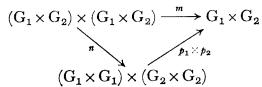
\includegraphics[keepaspectratio]{images/part002_baaabc67.jpg}}

where \(s(g, g') = (g', g)\) , \(m(g, g') = gg'\) , \(n(g, g') = g'g\) for all \(g\) , \(g'\) in \(G\) . This diagram is commutative. Hence \(n_*(t \otimes t') = m_*(s_*(t \otimes t')) = m_*(t' \otimes t)\) . This equality is precisely (i). Assertion (ii) follows from (i) and Proposition 6.

PROPOSITION 8. Let G, H be Lie groups and \(\phi\) a morphism of G into H. If \(t \in \mathcal{T}^{(\infty)}(G)\) , then \(\phi_{*}(t^{\vee}) = (\phi_{*}(t))^{\vee}\) .

Let \(\theta\) (resp. \(\theta'\) ) be the mapping \(g \mapsto g^{-1}\) of G into G (resp. of H into H). Then \(\phi \circ \theta = \theta' \circ \phi\) , whence \(\phi_*(\theta_*(t)) = \theta'_*(\phi_*(t))\) .

PROPOSITION 9. Let \(\mathrm{G}_1, \cdots, \mathrm{G}_n\) be Lie groups and \(\mathrm{G} = \mathrm{G}_1 \times \cdots \times \mathrm{G}_n\) . If the vector spaces \(\mathcal{T}^{(\infty)}(\mathrm{G})\) and \(\mathcal{T}^{(\infty)}(\mathrm{G}_1) \otimes \cdots \otimes \mathcal{T}^{(\infty)}(\mathrm{G}_n)\) are canonically identified, the algebra \(\mathcal{T}^{(\infty)}(\mathrm{G})\) is the tensor product of the algebras \(\mathcal{T}^{(\infty)}(\mathrm{G}_1), \ldots, \mathcal{T}^{(\infty)}(\mathrm{G}_n)\) . If \(t_i \in \mathcal{T}^{(\infty)}(\mathrm{G}_i)\) for \(i = 1, \ldots, n\) , then

\[
\left(t _ {1} \otimes \dots \otimes t _ {n}\right) ^ {\vee} = t _ {1} ^ {\vee} \otimes \dots \otimes t _ {n} ^ {\vee}.
\]

It suffices to consider the case \(n = 2\) . Let \(t_1, t_1'\) be in \(\mathcal{T}^{(\infty)}(\mathrm{G}_1)\) , \(t_2, t_2'\) in \(\mathcal{T}^{(\infty)}(\mathrm{G}_2)\) . We need to show that \((t_1 \otimes t_2) * (t_1' \otimes t_2') = (t_1 * t_1') \otimes (t_2 * t_2')\) and that \((t_1 \otimes t_2)^{\vee} = t_1^{\vee} \otimes t_2^{\vee}\) . Consider the diagram

\pandocbounded{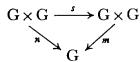
\includegraphics[keepaspectratio]{images/part002_69e6a490.jpg}}

where \(m((x_1, x_2), (x_1', x_2')) = (x_1x_1', x_2x_2')\) ,

\[
n ((x _ {1}, x _ {2}), (x _ {1} ^ {\prime}, x _ {2} ^ {\prime})) = ((x _ {1}, x _ {1} ^ {\prime}), (x _ {2}, x _ {2} ^ {\prime})),
\]

\(p_1(x_1, x_1') = x_1x_1', p_2(x_2, x_2') = x_2x_2'\) . This diagram is commutative. Hence

\[
m _ {*} \left(\left(t _ {1} \otimes t _ {2}\right) \otimes \left(t _ {1} ^ {\prime} \otimes t _ {2} ^ {\prime}\right)\right) = \left(p _ {1} \otimes p _ {2}\right) _ {*} \left(n _ {*} \left(\left(t _ {1} \otimes t _ {2}\right) \otimes \left(t _ {1} ^ {\prime} \otimes t _ {2} ^ {\prime}\right)\right)\right),
\]

that is

\[
\begin{array}{r l} (t _ {1} \otimes t _ {2}) * (t _ {1} ^ {\prime} \otimes t _ {2} ^ {\prime}) & = (p _ {1} \otimes p _ {2}) _ {*} ((t _ {1} \otimes t _ {1} ^ {\prime}) \otimes (t _ {2} \otimes t _ {2} ^ {\prime})) \\ & = p _ {1 *} (t _ {1} \otimes t _ {1} ^ {\prime}) \otimes p _ {2 *} (t _ {2} \otimes t _ {2} ^ {\prime}) \\ & = (t _ {1} * t _ {1} ^ {\prime}) \otimes (t _ {2} * t _ {2} ^ {\prime}). \end{array}
\]

It is seen analogously that \((t_1\otimes t_2)^\vee = t_1^\vee \otimes t_2^\vee\)

PROPOSITION 10. Let H be a Lie subgroup of G and \(i: \mathrm{H} \to \mathrm{G}\) the canonical injection. Then \(i_*\) is an injective homomorphism of the algebra \(\mathcal{T}^{(\infty)}(\mathrm{H})\) into the algebra \(\mathcal{T}^{(\infty)}(\mathrm{G})\) and \(i_*(t^\vee) = (i_*(t))^{\vee}\) for all \(t \in \mathcal{T}^{(\infty)}(\mathrm{H})\) .

This follows from Propositions 6 and 8 and Differentiable and Analytic Manifolds, R, 13.2.3.

\(\mathcal{T}^{(\infty)}(H)\) is identified with a subalgebra of \(\mathcal{T}^{(\infty)}(G)\) by means of the isomorphism of Proposition 10.

Remark. Proposition 10 remains valid if H is a Lie quasi-subgroup.

We recall (Differentiable and Analytic Manifolds, R, 13.5.1) that, if V is an analytic manifold over K, \(\mathcal{T}^{(\infty)}(\mathrm{V})\) has canonically a cogebra structure over K with a counit; the counit is the linear mapping of \(\mathcal{T}^{(\infty)}(\mathrm{G})\) into K which associates with each element of \(\mathrm{T}_x^{(\infty)}(\mathrm{V})\) its constant term.

PROPOSITION 11. Let G be a Lie group.

\begin{enumerate}
\def\labelenumi{(\roman{enumi})}
\item
  The cogebra \(\mathcal{T}^{(\infty)}(\mathbf{G})\) , with convolution, is a bigebra (Algebra, Chapter III, § 11, no. 4).
\item
  Let \(c\) be the coproduct on \(\mathcal{T}^{(\infty)}(\mathbf{G})\) . Let \(t \in \mathcal{T}^{(\infty)}(\mathbf{G})\) and write
\end{enumerate}

\[
c (t) = \sum_ {i = 1} ^ {n} t _ {i} \otimes t _ {i} ^ {\prime}.
\]

Then \(c(t^{\vee}) = \sum_{i=1}^{n} t_{i}^{\vee} \otimes t_{i}^{\prime\vee}\) .

We prove (i). In the definition of bigebras referred to, condition (1) follows from Propositions 2 and 3 and condition (2) follows from Differentiable and Analytic Manifolds, R, 13.5.1. Let \(d\) be the mapping \(g \mapsto (g, g)\) of G into \(\mathrm{G} \times \mathrm{G}\) . Then \(c = d_{*}\) and hence \(c\) is an algebra morphism (Propositions 6 and 9), which is condition (3). Let \(t \in \mathrm{T}_{g}^{\infty}(\mathrm{G})\) , \(t' \in \mathrm{T}_{g'}^{\infty}(\mathrm{G})\) have no constant term and \(\lambda\) , \(\lambda'\) be elements of K; then \(\varepsilon_{g} \otimes t'\) , \(t \otimes \varepsilon_{g'}\) , \(t \otimes t'\) are without constant term (Differentiable and Analytic Manifolds, R, 13.4.1) and hence the constant term of \((\lambda\varepsilon_{g} + t) * (\lambda' \varepsilon_{g'} + t')\) is \(\lambda\lambda'\) ; hence condition (4) holds.

We prove (ii). By Propositions 8 and 9,

\[
c (t ^ {\vee}) = d _ {*} (t ^ {\vee}) = (d _ {*} (t)) ^ {\vee} = \left(\sum_ {i = 1} ^ {n} t _ {i} \otimes t _ {i} ^ {\prime}\right) ^ {\vee} = \sum_ {i = 1} ^ {n} t _ {i} ^ {\prime \vee} \otimes t _ {i} ^ {\vee}.
\]

PROPOSITION 12. Let G, H be two Lie groups and \(\phi\) a morphism of G into H. Then \(\phi_{*}\) is a bigebra morphism of \(\mathcal{T}^{(\infty)}(G)\) into \(\mathcal{T}^{(\infty)}(H)\) .

This follows from Proposition 6 and Differentiable and Analytic Manifolds, R, 13.5.1.

Let \(G\) be a Lie group. The restrictions of the convolution and the coproduct to \(U(G)\) define a bigebra structure on \(U(G)\) . We have \(U(G)^{\vee} = U(G)\) . If \(\phi: G \to H\) is a Lie group morphism, we denote by \(U(\phi)\) the mapping \(t \mapsto \phi_{*}(t)\) of \(U(G)\) into \(U(H)\) ; this is a bigebra morphism. If \(\psi: H \to L\) is another Lie group morphism, then \(U(\psi \circ \phi) = U(\psi) \circ U(\phi)\) . If \(\phi\) is an immersion (resp. a submersion), \(U(\phi)\) is injective (resp. surjective) by Differentiable and Analytic Manifolds, R, 13.2.3. In particular, if \(H\) is a Lie subgroup of \(G\) , \(U(H)\) is identified with a subalgebra of \(U(G)\) , the coproduct on \(U(H)\) being the restriction of the coproduct on \(U(G)\) . If \(H\) is open in \(G\) , then \(U(H) = U(G)\) . If \(G_1, G_2\) are Lie groups, \(U(G_1 \times G_2)\) is identified with \(U(G_1) \times U(G_2)\) . The primitive elements of \(U(G)\) are those of \(T_e(G)\) (Differentiable and Analytic Manifolds, R, 13.5.3).

Again let \(\phi: \mathrm{G} \to \mathrm{H}\) be a Lie group morphism. If \(\operatorname{gr} \mathrm{U}(\mathrm{G})\) is identified \(\mathrm{TS}(\mathrm{T}_e(\mathrm{G}))\) and \(\operatorname{gr} \mathrm{U}(\mathrm{H})\) with \(\mathrm{TS}(\mathrm{T}_e(\mathrm{H}))\) , then \(\operatorname{gr} \mathrm{U}(\phi)\) is identified with \(\mathrm{TS}(\mathrm{T}_e(\phi))\) (Differentiable and Analytic Manifolds, R, 13.3.5). We apply this to the isomorphism \(g \mapsto g^{-1}\) of \(\mathrm{G}\) onto \(\mathrm{G}^{\vee}\) ; then \(\mathrm{T}_e(\phi) = -1\) and hence

\[
t \in \mathrm{U} _ {s} (\mathrm{G}) \Rightarrow t ^ {\vee} \equiv (- 1) ^ {s} t \bmod \mathrm{U} _ {s - 1} (\mathrm{G}).\tag{3}
\]

